\documentclass[11pt]{article}
\usepackage[margin=1in]{geometry}
\usepackage{amsmath,amssymb}
\usepackage{booktabs}
\usepackage{listings}
\usepackage{xcolor}
\usepackage{hyperref}
\hypersetup{colorlinks=true,linkcolor=blue,urlcolor=blue}

\lstset{
  basicstyle=\ttfamily\footnotesize,
  breaklines=true,
  breakatwhitespace=false,
  columns=fullflexible,
  frame=single,
  framesep=4pt,
  backgroundcolor=\color{gray!8},
  postbreak=\mbox{\textcolor{gray}{$\hookrightarrow$}\space},
}

\newcommand{\nats}{\,\text{nats}}
\title{Fully branch-wise DTL rates on the archaeal big tree:\\
likelihood landscape, best fit, cross-validation, and a reproducible protocol}
\author{gpurec / AleRax comparison --- This\_study / Undine C60}
\date{\today}

\begin{document}
\maketitle

\begin{abstract}
We re-analyse the rooting of the archaeal ``big tree'' (This\_study / Undine C60: 257
taxa, $S=513$ species-tree branches, 7{,}059 gene families given as ALE conditional-clade
distributions) with \texttt{gpurec}, a GPU re-implementation of AleRax's
duplication--transfer--loss (DTL) gene-tree/species-tree reconciliation. \texttt{gpurec}
reproduces AleRax's per-family log-likelihoods to Pearson $r=0.999998$. Allowing the DTL
rates to vary \emph{freely along every branch} ($\sim$2{,}000 free parameters) recovers the
same \textbf{Euryarchaeota} root as AleRax and the same ancestral (LACA) gene content, with
duplication/transfer rates that are essentially clade-constant and loss rates that are
branch-heterogeneous. The free per-branch model is the highest-likelihood fit found, and
held-out cross-validation shows its advantage \emph{generalises} (it is not overfitting).
The likelihood surface has (at least) three basins; the global optimum (Euryarchaeota) is
reached by warm-starting from a clade-grouped fit, but is missed by every cold (uniform)
initialisation we have tried. We document the reproducible protocol and the open
cold-start problem.
\end{abstract}

\section{Setup and engine fidelity}
\label{sec:setup}
The species tree has $S=513$ branches; the data are 7{,}059 gene families
(\texttt{.ale} conditional-clade distributions built from UFBoot samples). Everything is
in $\log_2$ (bits) space internally; rates reported here are natural rates, and
log-likelihoods are in \emph{nats} (natural log) unless noted. Fraction-missing is handled
in the AleRax-faithful \texttt{e-only} mode.

\paragraph{Engine fidelity.} Evaluated at AleRax's \emph{exact} per-branch rates,
\texttt{gpurec}'s per-family log-likelihoods match AleRax's
(\texttt{per\_fam\_likelihoods.txt}) to \textbf{Pearson $r=0.999998$} for every candidate
root and every AleRax model class (\texttt{global}, \texttt{DTL\_br2},
\texttt{DTL\_br1\_O}), up to a constant per-family offset. The engine is therefore not in
question; the discussion below concerns the \emph{optimiser} and the \emph{model richness}.

\section{The likelihood landscape: three basins}
\label{sec:basins}
Fitting the rates by maximum likelihood reveals a multi-modal surface. Table~\ref{tab:basins}
summarises the three basins we observe (total data log-likelihood, natural log, Eury-rooted
unless noted). The deciding coordinate is the \emph{origination} distribution $O$ (where
gene families are born on the tree): a deep, concentrated $O$ gives Euryarchaeota; a diffuse
$O$ gives a near-tie or the small-genome-attraction (SGA) artifact.

\begin{table}[h]
\centering
\begin{tabular}{lrl}
\toprule
Basin & data $\log L$ (nats) & how reached \\
\midrule
Deep / Euryarchaeota (best) & $-1{,}631{,}537$ & warm-start from clade-grouped fit \\
Cold near-tie               & $-1{,}664{,}248$ (Eury) & cold global-rate warm-up \\
Cold SGA stall              & $\approx -1{,}712{,}000$ & cold uniform initialisation \\
\bottomrule
\end{tabular}
\caption{Three basins of the big-tree likelihood. The deep/Euryarchaeota basin is the
global optimum found, $\sim$33k nats above the cold near-tie and $\sim$80k above the cold
SGA stall. In the cold near-tie basin the SGA root Cluster2 ($-1{,}663{,}618$) marginally
\emph{edges} Eury ($-1{,}664{,}248$); only in the deep basin does Eury win decisively. The
initialisation selects the basin.}
\label{tab:basins}
\end{table}

\paragraph{Why cold fails.} At full ML the deep basin is the global maximum, but it has a
\emph{small basin of attraction}: from a uniform initialisation the optimiser converges to
the near-tie or SGA basin and never climbs to the deep one. The deep basin requires the
origination $O$ \emph{and} the DTL rates to be jointly near the AleRax solution --- they are
coupled --- which is why a joint warm-start works and partial seeds do not
(\S\ref{sec:cold}).

\section{The best fit: fully branch-wise (FULLbasin)}
\label{sec:bestfit}
The best fit is a \emph{fully free per-branch} model: every branch has its own duplication,
loss and transfer rate plus its own origination weight ($\sim$2{,}000 free parameters),
warm-started from the clade-grouped fit. It attains
$\log L = -1{,}631{,}537\nats$, the highest found, $\sim$11k nats above the clade-grouped fit.

\paragraph{Rooting.} Euryarchaeota is rank 1 by $+3{,}568\nats$ over the next root; the deep
clades \{Eury, TackA, DPANN\} sit at the top and the small-genome roots at the bottom
(Cluster2 is $-12{,}190\nats$ below Eury).

\paragraph{AU test.} A Shimodaira approximately-unbiased (AU) test over all 15 candidate
roots, on the free per-branch per-family likelihoods, places \textbf{Euryarchaeota alone}
in the 0.05 confidence set (BP$=1.0$); every other root, \emph{including MHH}
($-1{,}637{,}704$, rank 4, $-6{,}167\nats$ behind Eury), is rejected (AU$\approx 0$).
By contrast AleRax's parsimonious \texttt{DTL\_br2} model gives a \emph{region}
\{Euryarchaeota, MHH\} (MHH only 9.7 nats behind). The free model is therefore
\emph{sharper}; we read this as the consequence of model richness plus the warm-start, not
as stronger evidence (see \S\ref{sec:cv} for why it is nonetheless not overfitting).

\paragraph{Rate structure (Fig.~\ref{fig:violin}).} With rates free to vary, duplication and
transfer come out essentially \emph{clade-constant} --- clade membership (the paper's 23
DTL classes) explains $R^2\approx 0.94$ of their variance --- whereas loss is
\emph{branch-heterogeneous}: only $R^2\approx 0.38$ of its variance is clade-level. Most of
the free model's $\sim$11k-nat advantage over clade-grouping lives in the loss rates.

\paragraph{Origination.} The fitted $O$ is concentrated but free: two branches carry
$\sim$32\% of the origination mass (top branch $0.19$), over a near-uniform diffuse floor
(73 branches hold 50\%, 279 hold 90\% of the mass).

\paragraph{Ancestral genome (LACA, Fig.~\ref{fig:laca}).} Of the 7{,}059 families, the free
model places \textbf{903} at the root and the clade-grouped (AleRax) rates \textbf{772}
(thresholded at posterior $\ge 0.5$); \textbf{722} are shared (Jaccard $0.76$), and the
per-family origination-at-root probabilities correlate $r=0.96$. The free model reconstructs
a somewhat larger ancestral genome.

\begin{figure}[h]\centering
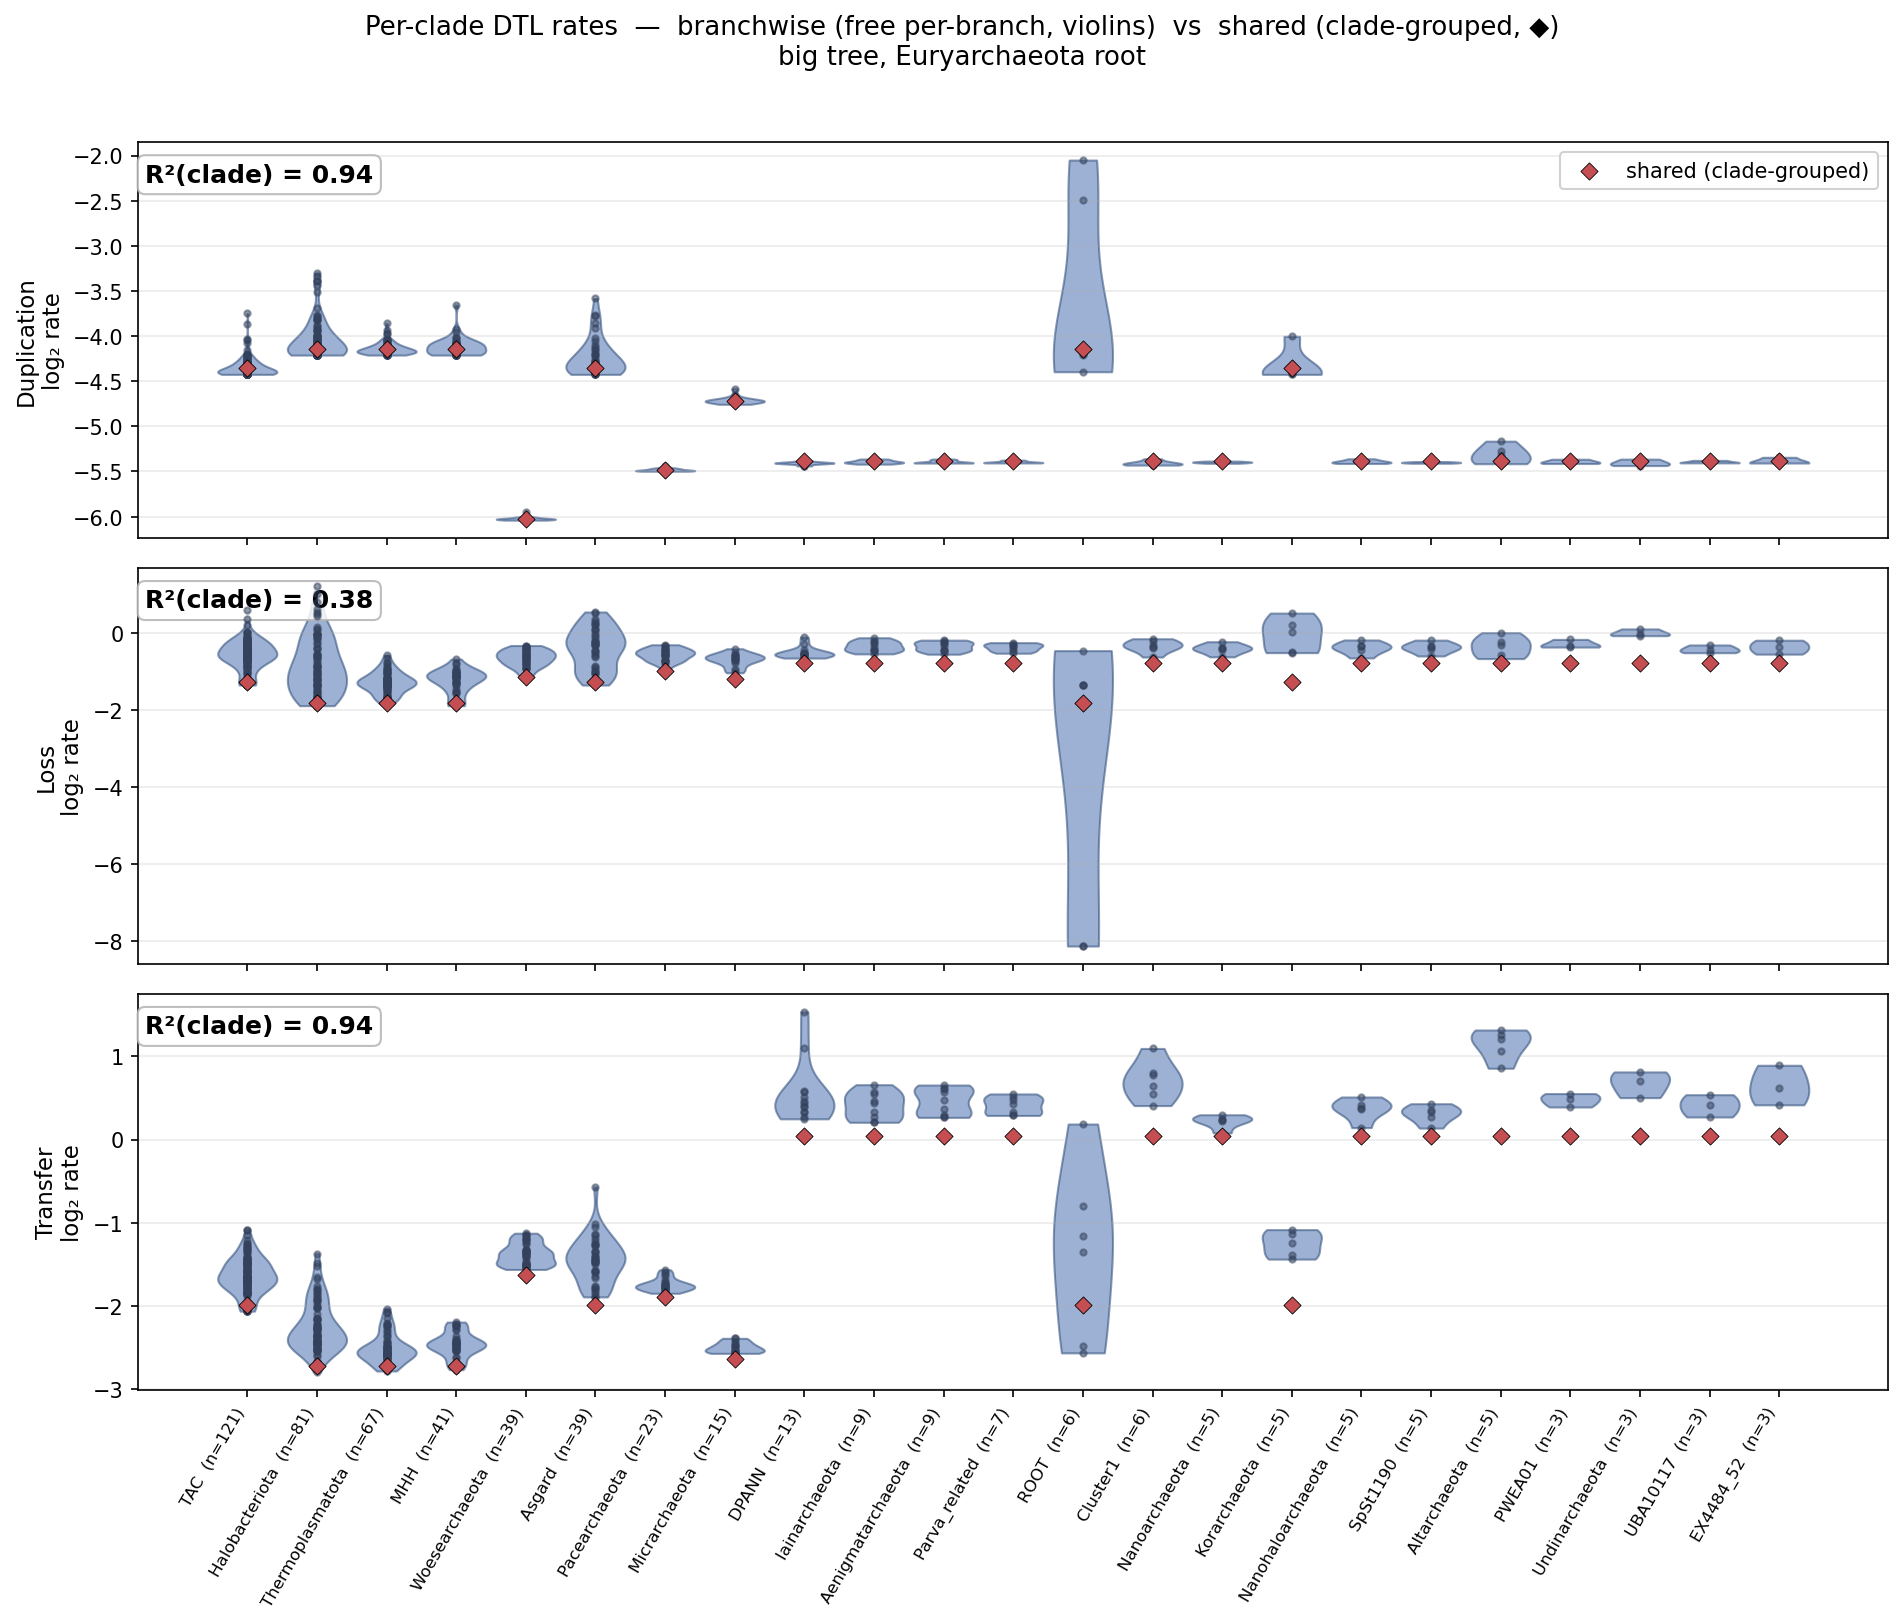
\includegraphics[width=0.95\textwidth]{rate_violin_bigtree_Eury.png}
\caption{Per-clade DTL rates: branchwise (free per-branch, blue violins) vs.\ shared
(clade-grouped, red $\blacklozenge$), one panel per rate. D and T violins are tight around
the shared rate ($R^2\approx 0.94$); L violins are wide ($R^2\approx 0.38$).}
\label{fig:violin}
\end{figure}

\begin{figure}[h]\centering
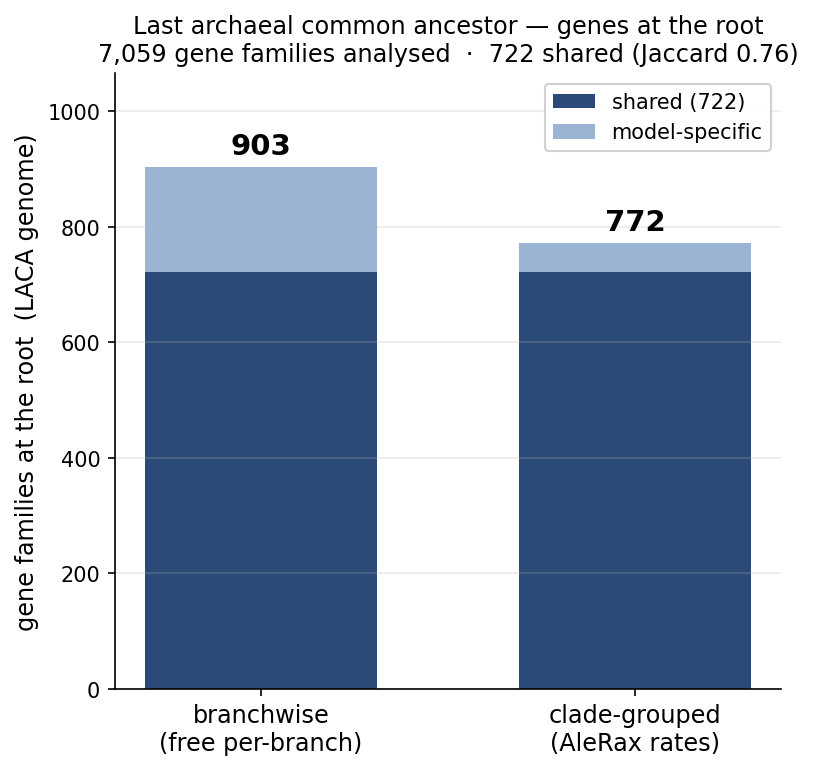
\includegraphics[width=0.55\textwidth]{laca_families_bigtree_Eury.png}
\caption{Gene families at the root (LACA): 903 under the free per-branch model vs.\ 772
under clade-grouped (AleRax) rates; 722 shared (Jaccard 0.76), of 7{,}059 analysed.}
\label{fig:laca}
\end{figure}

\section{Cross-validation: the richness is not overfitting}
\label{sec:cv}
To test whether the $\sim$2{,}000 free parameters fit noise, we fit both the clade-grouped
and the free per-branch model on a \emph{training half} (first 3{,}530 families) and scored
the \emph{held-out half} (3{,}529 families never used in fitting).

\begin{table}[h]
\centering
\begin{tabular}{lrrrr}
\toprule
model & train $\sum\log L$ & held-out $\sum\log L$ & train/fam & held-out/fam \\
\midrule
free (per-branch)   & $-1{,}373{,}618$ & $-257{,}725$ & $-389.13$ & $-73.03$ \\
grouped (clade)     & $-1{,}383{,}170$ & $-259{,}280$ & $-391.83$ & $-73.47$ \\
\midrule
free $-$ grouped    & $+9{,}551$ & $\mathbf{+1{,}556}$ & & $+0.44$ \\
\bottomrule
\end{tabular}
\caption{Held-out cross-validation (Eury root). The free per-branch model beats the
clade-grouped model on \emph{held-out} families by $+1{,}556\nats$ ($+0.44$/family).
Overfit parameters would hurt out-of-sample; these help. The train advantage ($+9{,}551$)
shrinks to $+1{,}556$ held-out --- $\sim$5/6 of the in-sample gain is optimism, but the
remaining positive sixth generalises. \textbf{Verdict: not overfitting.}}
\label{tab:cv}
\end{table}

\noindent\textbf{Scope.} This establishes that the per-branch \emph{rate} richness
generalises (the crux of the overfitting concern). It does not separately cross-validate the
AU \emph{region} (which would require per-root refits). The index split is also family-size
unbalanced (train $-389$/fam vs.\ test $-73$/fam), so this is a generalisation test
\emph{across} a family-size shift; a random split would give a cleaner balanced number.

\section{Reproducible protocol (the minimal robust setup)}
\label{sec:protocol}
All commands run from the \texttt{gpurec-cpp} checkout on a single A100 (\texttt{largegpu}).
Paths use the cluster layout; \texttt{\$U} is the output directory, \texttt{\$DD} the data
root, \texttt{\$CG} the AleRax clade-grouping directory.

\begin{lstlisting}[language=bash]
U=/work/SzollosiU/gergely-szollosi/williams_run/undine
DD=/work/SzollosiU/gergely-szollosi/williams_run/data/3_Reconciliation/This_study
CG="$U/alerax_ref/3_Reconciliation/This_study/5_reconcilation models/DTL_br1_O/Undine_C60_Euryroot2_OR"
# data: tree  $DD/4_species_tree/Undine_C60_<ROOT>root_short_name.nw
#       .ale   $DD/3_UFBOOTs/ufboot_for_alerax/*.ale   (7059 families)
#       fraction_missing  $DD/fraction_missing
\end{lstlisting}

\paragraph{Step 1 --- clade-grouped warm-up (lands in the deep basin).}
Fits the paper's clade-grouped DTL plus origination, initialised from AleRax's rates. This
is the step that selects the deep/Euryarchaeota basin. ($\sim$30 min on one A100.)
\begin{lstlisting}[language=bash]
python experiments/run_undine_branchwise.py --root Eury \
  --families 0 --min-species 1 --fm-mode e-only --prior none \
  --clade-groups "$CG" --init-from-alerax --origination optimize \
  --family-batch-size 500 --steps 250 --dtype float64 \
  --out $U/AXgrp_DTL_br1_O_Eury.rates.txt
\end{lstlisting}

\paragraph{Step 2 --- fully free per-branch fit (the best fit).}
Warm-started from Step 1; no rate grouping, no prior, free per-branch origination.
($\sim$1--7.5 h on one A100, depending on convergence.)
\begin{lstlisting}[language=bash]
python experiments/run_undine_branchwise.py --root Eury \
  --families 0 --min-species 1 --fm-mode e-only --prior none \
  --origination optimize \
  --init-from-rates $U/AXgrp_DTL_br1_O_Eury.rates.txt.json \
  --family-batch-size 500 --steps 250 --dtype float64 \
  --out $U/FULLbasin_Eury.rates.txt
\end{lstlisting}

\paragraph{Step 3 --- rooting / AU over all 15 roots.}
Run Steps 1--2 for each root (substitute \texttt{--root} and the matching
\texttt{Undine\_C60\_<ROOT>root2\_OR} grouping dir), then:
\begin{lstlisting}[language=bash]
python experiments/au_fullbasin.py   # AU test on the FULLbasin per-root likelihoods
\end{lstlisting}

\paragraph{Step 4 --- ancestral genome (LACA) content.}
\begin{lstlisting}[language=bash]
python experiments/laca_compare.py --root Eury \
  --sidecar $U/FULLbasin_Eury.rates.txt.json \
  --out $U/laca_Eury.json
\end{lstlisting}

\paragraph{Step 5 --- overfitting cross-validation.}
Fit on the training half (\texttt{--families 3530}) for both models, then score held-out:
\begin{lstlisting}[language=bash]
# grouped on train half
python experiments/run_undine_branchwise.py --root Eury --families 3530 \
  --min-species 1 --fm-mode e-only --prior none --clade-groups "$CG" \
  --init-from-alerax --origination optimize --family-batch-size 500 \
  --steps 250 --dtype float64 --out $U/CVgrouped_Eury_train.rates.txt
# free per-branch on train half, warm-started from the grouped train fit
python experiments/run_undine_branchwise.py --root Eury --families 3530 \
  --min-species 1 --fm-mode e-only --prior none --origination optimize \
  --init-from-rates $U/CVgrouped_Eury_train.rates.txt.json \
  --family-batch-size 500 --steps 250 --dtype float64 \
  --out $U/CVfree_Eury_train.rates.txt
# held-out verdict
python experiments/cv_eval.py --root Eury --train-n 3530 \
  --free $U/CVfree_Eury_train.rates.txt.json \
  --grouped $U/CVgrouped_Eury_train.rates.txt.json \
  --out $U/cv_eval_Eury.json
\end{lstlisting}

\paragraph{Key flags.}
\texttt{--fm-mode e-only} (AleRax-faithful fraction-missing);
\texttt{--prior none} (no Brownian/TV smoothing; add \texttt{--dtl-tv-lambda <$\lambda$>} for
a fused-lasso that auto-groups the free rates);
\texttt{--origination optimize} (fit per-branch origination; the rooting signal);
\texttt{--clade-groups <dir>} + \texttt{--init-from-alerax} (clade-grouped model seeded from
AleRax --- the basin selector);
\texttt{--init-from-rates <sidecar>} (warm-start chain);
\texttt{--family-batch-size 500} (memory; the $S{=}513$, 7059-family forward must be batched);
\texttt{--dtype float64} (gradient accuracy);
\texttt{--families N} (use the first $N$ families; $0=$ all).

\section{Open problem: cold-start basin-finding}
\label{sec:cold}
The deep/Euryarchaeota basin is the global optimum but is only reached by warm-starting
(Steps 1--2). From a cold (uniform-origination) start, every strategy tried so far lands in
the near-tie or SGA basin:
\begin{itemize}
\item anti-concentration (Simpson) origination barrier --- directionally \emph{wrong}
(pushes $O$ toward uniform; sinks Euryarchaeota);
\item fixed root-mass / depth origination priors --- over-constrain and destroy the fit;
\item global-rate warm-up --- reaches only the near-tie ($-1{,}664$k);
\item fused-lasso (TV) annealing --- regularises the DTL, not the (bistable) $O$; stuck at
the near-tie;
\item structured-$O$ seed ($\omega \propto -\text{depth}$) --- diffuses straight back to the
near-tie.
\end{itemize}
The deep basin needs the structured $O$ \emph{and} the matching DTL together; a cold,
initialisation-independent route to it is unsolved. The most promising untried idea is a
\emph{deep-origination prior homotopy}: impose a strong root-region origination prior to put
the optimiser in the deep basin, then anneal the prior to zero (the unconstrained optimum it
then converges to should be the global/deep basin). This is the directionally-correct
counterpart of the failed anti-concentration barrier.

\end{document}
